
\section{Deterministic Queueing Networks}
\label{sec:determ-queu-netw}

\subsection*{Theory and Exercises}

\Opensolutionfile{hint}
\Opensolutionfile{ans}

Before we study queueing networks in stochastic settings, we should
familiarize ourselves with the behavior of networks of queueing
systems in the simplest setting possible.  This is, arguably, a network in which all servers have constant service times, which is the topic for this section.


A queueing network can be represented as a
\emph{graph}. \emph{Stations} form the \emph{nodes} in the graph, and
\emph{edges} between nodes represents the routing, which is the
possibility that jobs can move from one station to another. A simple
example is a network of $n$ stations in tandem. Jobs arrive at
station~1, and after service they move to station~2. Then they move to
station 3, and so on, until they leave the network after being served at
station~$n$.  A station can contain one or more servers. We assume that all servers have constant  job processing times. However, service times need not be equal for all servers.  

We need some more definitions. The \emph{raw processing time} $T_0$ is the minimal amount
of time  needed to move from the start of the system to the end. More precisely, it is the sum of the long-run average processing times of each workstation in the routing. The \emph{utilization} of station~$i$ is $\lambda_i/\mu_i$, i.e., the rate $\lambda_i$ at which work arrives divided by the processing rate of the server(s) at station~$i$. The \emph{bottleneck} station is the
station with the highest utilization. We write $r_b$ for the processing rate of the bottleneck station.  The \emph{critical  work in progress (WIP)}  $W_0$ is defined  as $W_0=r_b T_0$. This is the minimal amount of work required in the network to keep the bottleneck station fully loaded. To see how this relates to Little's law, observe that if jobs leave the network at rate $r_b$, they have to arrive at the network at rate $r_b$---we also assume that inter-arrival times are constant so that no explosions occur. Note that this is the largest arrival rate that the network can handle with queues growing to infinity. But then, with Little's law, the amount of work in the system is equal to the arrival rate times the time in the system.

In the next set of exercises we illustrate the above concepts by means of a network with $n$ single-server stations in tandem and all stations have the same service time $S$. 

\begin{exercise}
Suppose we would release just one job at a time in the above tandem system, that is,  only when a job has visited all stations, the next job is released. What is the throughput of the network?
\begin{solution}
In this case, the throughput $\mu$ of the network is $1/T_0$: only one server at a time is serving a job, the rest of the servers are forced to be idle as we only allow one job at a time in the network. 
\end{solution}
\end{exercise}

\begin{exercise}
Motivate that if we are prepared to release $w$ jobs, the throughput of the network becomes
\begin{equation*}
  \mu(w) = \min\{w, n\} \frac 1{T_0}.
\end{equation*}
Conclude that we need a minimal amount $w$ in the network to guarantee that
the network's throughput $\mu(w)$ exceeds the arrival rate $\lambda$, that is, there is a minimal $w$ such that $\mu(w) \geq \lambda$.
\begin{solution}
If there is one job in the system, $\mu(1) = 1/T_0$. If there are two, both jobs can be simultaneously worked on, each at  a different station, hence $\mu(2)=2/T_0$. And so on, until all stations are filled, at the same time, by a job, in which case $\mu(n) = n/T_0$. When there are yet more jobs in the network, only $n$ can be simultaneously in service, the rest must wait at some station.
\end{solution}
\end{exercise}


\begin{exercise}
Show that  only when $w\geq n$.
\begin{equation*}
\mu(w) = \frac 1S,
\end{equation*}
in which case the maximal capacity of the network is achieved.
\begin{solution}
\begin{equation*}
  \mu(w) = \frac{n}{T_0} = \frac{n}{n S} = \frac 1S.
\end{equation*}
\end{solution}
\end{exercise}

Thus, for given $w$  the largest arrival rate the network  can handle is  $\lambda = \mu(w)$, and the maximal rate at which it can process jobs is $r_b=1/S$. 

\begin{exercise}
  Show that when $\lambda=\mu(w)$,  the waiting time in the network is 
\begin{equation*}
  \E W = 
\begin{cases}
  T_0=n S, & \text{ if } w\leq n, \\
  \frac{w}{n} T_0 = w S, & \text{ if } w\geq n.
\end{cases}
\end{equation*}
\begin{hint}
  Use Little's law.
\end{hint}
  \begin{solution}
\begin{equation*}
  \begin{split}
  \E W 
= \frac{\E L}{\lambda} = \frac{w}{\mu(w)} = \frac{w}{\min\{w, n\}} T_0 
=
\begin{cases}
  T_0=n S, & \text{ if } w\leq n, \\
  \frac{w}{n} T_0 = w S, & \text{ if } w\geq n.
\end{cases}
  \end{split}
\end{equation*}
  \end{solution}
\end{exercise}

\begin{exercise}
  What do you conclude from the above exercises?
  \begin{hint}
   If $w<n$, then what happens? If $w>n$, what are the $w-n$ jobs doing?
  \end{hint}
  \begin{solution}
When $w>n$, there must be $w-n$ jobs in queue and the
other $n$ jobs are in service. So, in conclusion, in deterministic
tandem networks adding more than $n$ jobs does not increase the
network's throughput, but only increases the waiting times. On the other
hand, setting $w<n$ minimizes the waiting times, but also negatively
affects the throughput of the network. 
  \end{solution}
\end{exercise}

In conclusion, to balance waiting times and throughput, we need to tune the amount of work in the system. The critical WIP $W_0$ is the minimal WIP we need to keep all bottleneck machines occupied without adding extra waiting time. Jobs can never pass through  the network in less time than $T_0$, and the maximal output rate of the network is $r_b = 1/S$. Thus, 
\begin{align}\label{eq:t0}
T_0&= n S, & r_b&= 1/S, & W_0 = r_b T_0 = n.
\end{align}

The problems below are generalizations to networks with multi-server
stations, servers with different processing rates, and multiple
routings. They are meant to help you become acquainted with networking
behavior, and also with Little's law, which we use time and again
here\footnote{Warning, these problems are quite challenging, despite their apparent simplicity; I had much less trouble making the problems than solving them. In fact, to ensure that
I got the answer right, I often tried to find at least two different ways to
solve the same problem.}.

\begin{exercise}
  A production system consists of 2 separate stations. Jobs never go
  from one machine to another. The processing times are
  $(t_1, t_2) = (1, 2)$ hours. The arrival rates are
  $(\lambda_1, \lambda_2) = (1/3, 1/3)$ per hour. What is the fastest
  machine? Which machine is the bottleneck? 
  \begin{solution}
    The processing rates are $\mu_1=1/1$ and $\mu_2 = 1/2$ per hour,
    respectively. The utilizations $\rho_i=\lambda_i/\mu_i$ are $1/3$
    and $2/3$, respectively. Thus, machine 2 is the bottleneck: it has
    the highest utilization.
  \end{solution}
\end{exercise}

\begin{exercise}
In the network of the previous exercise, what are $T_0$ and $W_0$? 
  \begin{solution}
Since these machines are not related by a routing (jobs going from
    one machine to another), computing $T_0$ and so on does not make
    much sense for the network. We can just consider each machine on
    its own. As we need $2$ jobs to keep each machine busy, it
    follows that $W_0=2$. 

We can use Little's law to find $T_0$. The rate at which jobs can be served is $\mu = 1+1/2 = 3/2$. Thus, 
\begin{equation*}
  T_0 = W_0/\mu = 2/(3/2)=4/3.
\end{equation*}
Clearly, the average time a job spends in this system is $4/3$ time units
if jobs arrive at the rate they are served. (Recall, everything is
deterministic.)

Can we see this in another way? Yes, because $2$ out of $3$ jobs have service time of $1$, and $1$ out of $3$ a service time of $2$,
\begin{equation*}
  \frac23 1 + \frac 1 3 2 = \frac 4 3.
\end{equation*}
  \end{solution}
\end{exercise}



\begin{exercise}
  A production network consists of 3 single-machine stations in
  tandem, i.e., in series, like the sketch below.  The
  processing times are $(2, 3, 2)$ hours respectively, i.e., constant
  and such that $t_1=2$ hours, $t_2=3$ hours and $t_3=2$ hours.
What are the critical WIP $W_0$, bottleneck
  capacity $r_b$ and raw processing time~$T_0$?

    \centering
    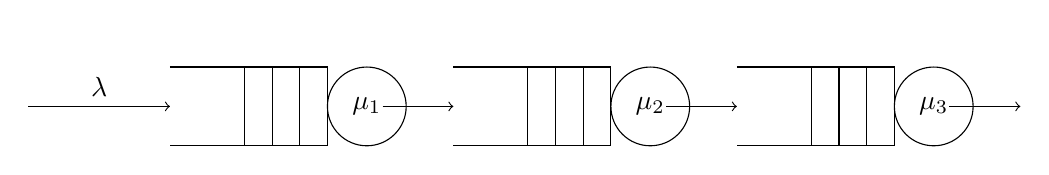
\begin{tikzpicture}[xscale=0.9,
->-/.style={decoration={markings, mark=at position .5 with {\arrow{stealth}}},
postaction={decorate}},
queuei/.pic={
  \draw%[line width=1pt]
    (0,-0.5) -- ++(2cm,0) -- ++(0,-1cm) -- ++(-2cm,0);
   \foreach \Val in {1,...,3}
     \draw ([xshift=-\Val*10pt]2cm,-0.5) -- ++(0,-1cm);
\draw (2.5,-1) circle [radius=0.5cm] node {#1};}
]
\path 
  (0,1) pic {queuei=$\mu_1$}
  (4,1) pic {queuei=$\mu_2$}
  (8,1) pic {queuei=$\mu_3$};

\draw[->] (-2,0)--(0,0) node[midway, anchor=south] {$\lambda$};
\draw[->] (3,0)--(4,0); 
\draw[->] (7,0)--(8,0); 
\draw[->] (11,0)--(12,0); 
%\draw[->-] (2.5,-0.5)-- ++(0,-1) -- ++(5.,0) -- ++(0, 1.5); 

\end{tikzpicture}

  \begin{solution} 
    The raw processing time is just the sum of the processing times at
    each station. All stations have the same arrival rate, hence
    machine, being the slowest, is the bottleneck. Hence,
 \begin{align*}
      T_0 &= 2 + 3 + 2 = 7\\
   r_b &= \mu_2 = \frac13 \\
      W_0 &= r_b T_0 = \frac73.
    \end{align*}
  \end{solution}
\end{exercise}

\begin{exercise}
  A production network consists of 3 single-machine stations in tandem
  with processing times $(2, 3, 2)$ hours.  Suppose we modify this
  network by adding one extra machine to station 2, with processing
  time $t=3$ hours.  What are $W_0$, $r_b$ and $T_0$?
  \begin{hint}
Is the new machine placed in parallel or in series?
  \end{hint}
  \begin{solution}
    Realize that machines at a station are in parallel, not in
    series. Thus, when we add capacity to station 2, we don't add an
    extra processing step to station 2, we increase capacity. 

    Now 
    \begin{equation*}
      r_2 = \frac13 + \frac13 = \frac 23,
    \end{equation*}
    so that station 2 is no longer the bottleneck. Station 1 and
    station 3 are the bottlenecks.
    \begin{align*}
      r_b &= \frac12 \\
      T_0 &= 2 + 3 + 2 = 7\\
      W_0 &= r_b T_0 = \frac72.
    \end{align*}

    Often, students think that the processing rate is the inverse of
    the processing time, i.e., $t=r^{-1}$. This is not the case for
    multi-server stations. Thus, realize that the raw processing time
    at station 2 is still $3$ hours, not $3/2$.
  \end{solution}
\end{exercise}


\begin{exercise}
  A production network consists of 3 single-machine stations in tandem
  with processing times $(2, 3, 2)$ hours.  Suppose we modify this
  network by adding one extra machine to station 2 with
  processing time $t=4$ hours.  What are $W_0$, $r_b$ and $T_0$?
  \begin{hint}
Check your reasoning very carefully here. It is easy to do it wrong.
  \end{hint}
\begin{solution}
Now, 
\begin{equation*}
  r_2 = \frac13 + \frac 14 = \frac 7{12} > \frac12,
\end{equation*}
hence, station 1 and 3 are bottlenecks. 


However, $t_2$ cannot be $3$ hours anymore: some jobs will spend 4
hours at station 2 rather than 3 hours. In fact, the computation of
the raw processing time at station 2, $t_2$ say, is a bit tricky. Some
students reason that both machines serve half of the jobs, so that
$T_2=(3+4)/2$ hours.  This, however, is not quite realistic. Like
this, you would load the slow machine all of the time, and the faster
machine would be idle quite a bit of the time. 


  Rather than spreading the jobs evenly over the two machines, we can
  also assume that each machine takes in work in proportion to its
  processing rate.  Then we reason like this. Consider 12 hours. In
  those 12 hours, the slow machine processes 3 jobs with duration 4
  and the fast machine processes 4 jobs with duration 3. Therefore:
  \begin{equation*}
    t_2 = \frac 3 7 4 + \frac 4 7 3 = \frac{24}7.
  \end{equation*}
  Another way to get this is like this. We can `stuff' station 2 with
  jobs. The most jobs that fit in simultaneously is 2, one job per
  machine. Then, with Little's law,
  \begin{equation*}
   t_2 = \frac{W}{r_2} = \frac{2}{7/12} = \frac{24}7,
  \end{equation*}
i.e., the same as the other answer.

Now, finally, 
    \begin{align*}
      r_b &= \frac12 \\
      T_0 &= 2 + \frac{24}7 + 2 = 4 + 3 + \frac37 = 7 \frac37\\
      W_0 &= r_b T_0.
    \end{align*}

    Finally, and the most realistic, is that the fast machine is
    always working, and the slow machine covers the rest.  In that
    case, suppose that the fast machine processes jobs at rate $r_1$
    and the slow at rate $r_2$. Then, since jobs arrive with rate
    $r_a$, the fast machine processes a fraction of $r_1/r_a$ of the
    jobs, and the slow machine processes the leftovers, i.e., a
    fraction of $(r_a-r_1)/r_a$ of the jobs. The raw processing time then becomes
    \begin{equation*}
      \begin{split}
      t_2 
&= \frac{r_1}{r_a} t_1 + \frac{r_a-r_1}{r_a} t_2 \\
&= \frac{1/3}{1/2} 3 + \frac{1/2-1/3}{1/2} 4 \\
&= 2 + \frac{1/6}{1/2} 4 \\
&= 2 + \frac{4}{3} = 3\frac13,
      \end{split}
    \end{equation*}
and then,
\begin{equation*}
  T_0 = 2 + t_2 + 2 = 7\frac13,
\end{equation*}
and this is a tiny bit less than the previous way of organizing things. 

So, why are the above answers different? One reason is that the
objective is not explicitly stated. It might be that, to minimize time
in a multi-server station, it is optimal to let a fast machine idle
and wait until the next job comes in. If we were to assign this next
job to a slow machine, the time in the system may be longer.  In
general, it might be that schedules that minimize $T_0$ (on average)
are not work-conserving (i.e., such that when jobs are waiting, not
all machines are idle.)
\end{solution}
\end{exercise}


\begin{exercise}
Why does the critical WIP change in the different cases above? 
\begin{solution}
  Because $T_0$ increases and/or the bottleneck rate increases. In
  both cases, we need more $W_0$ to fill the network and achieve that
  the throughput can be equal to $r_b$ in the best case.
\end{solution}
\end{exercise}

\begin{exercise}
  A production network consists of 3 single-machine stations in tandem
  with processing times $(2, 3, 2)$ hours.  Suppose we modify this
  network by adding one extra machine to station 2 with 
  processing time $t=1$ hour.  What are $W_0$, $r_b$ and $T_0$?
\begin{solution}
  Now the slow machine at station 2 becomes superfluous. The fast
  machine at station 2 can cope with all jobs that arrive from station
  1.
    \begin{align*}
      r_b &= \frac12 \\
      T_0 &= 2 + 1 + 2 = 5\\
      W_0 &= r_b T_0.
    \end{align*}

    Thus, why would you assign part of the jobs to the slow machine at
    station 2? There is no queue, the fast machine can cope with all
    the jobs. Moreover, assigning any job to the slow machines just
    adds to the cycle time.

Taking  $T_2=(1+3)/2=2$ is plainly silly. 
\end{solution}
\end{exercise}

\begin{exercise}
  In the previous question, it might seem that one machine at the
  second station is superfluous. Which one, and why? Would you remove
  this superfluous machine in a real production network?
\begin{solution}
  See above. I would not remove the slow machine. In real life there
  is variability: the fast machine might fail for instance. Spare
  capacity is useful. However, if it is very costly to keep the slow
  machine operational, I would scrap it.
\end{solution}
\end{exercise}


% What would you have
% said if the processing time of the slow machine would have been 5
% hours? Then you simply cannot give half of the jobs to the slow
% machine; it will overflow.

\begin{exercise}
  A production network consists of 3 single-machine stations in tandem
  with processing times $(2, 3, 2)$ hours.  Suppose we modify this
  network by adding one extra machine to station 2 with processing
  time $t=7$ hours.  What are $W_0$, $r_b$ and $T_0$?
\begin{solution}
  \begin{align*}
  r_2 &= \frac13 + \frac17 = \frac{10}{21} < \frac12\\
\intertext{hence station 2 is still the bottleneck}
T_2 &= \frac{3}{10}7 + \frac{7}{10}3 = \frac{42}{10}=\frac{21}{5}\text{hour}\\
T_0&=2+\frac{21}{5} +2\\
r_b &= \frac{10}{21}\\
W_0 &= r_b T_0.
   \end{align*}

   Note that we add capacity, so that we can process more jobs per
   unit time, but the raw processing time increases!
\end{solution}
\end{exercise}


\begin{exercise}
  A production network consists of 3 single-machine stations in tandem
  with processing times $(2, 3, 2)$ hours.  Suppose we modify this
  network such that $2/3$ of the jobs \emph{ leave after the first}
  station, i.e., between station 1 and 2.  What are $W_0$, $r_b$ and
  $T_0$? 
\begin{solution}
  Now there are two loops. One third of the jobs pass all three
  stations. Station 1 can process these job at rate 
  \begin{equation*}
\frac13 r_1 = \frac 13 \frac 12=\frac 16
  \end{equation*}
  per hour. Since this is smaller than $r_2$ and $r_3$, station 1 is
  the bottleneck rate for this loop. Thus, $W_0$ in this loop is
  $r_b T_0 = 1/6\cdot 7 = 7/6$.

  The other loop only contains station 1. The bottleneck rate in this
  loop is 
  \begin{equation*}
r_1\frac23 = \frac12\frac23 = \frac13. 
  \end{equation*}
Thus,
  $W_0 = r_b T_0 = 1/3\cdot 2 = 2/3$ for this loop. 

Hence, the total WIP is $7/6 + 2/3 = 11/6$ and
\begin{equation*}
T_0 = \frac13  7 + \frac 23  2=\frac{11}3,
\end{equation*}
since $1/3$ take the long loop with $T=7$ and $2/3$ the short loop
with $T=2$. Thus, $T_0$ is the weighted average raw processing time.

Another way to analyze this situation is like this. Station 1 is the
bottleneck, because its utilization is 1, while
\begin{align*}
  \rho_2 &= \lambda_2 t_2 = \frac12\frac13 3 = \frac 12\\
  \rho_3 &= \lambda_3 t_3 = \frac12\frac13 2 = \frac 13.
\end{align*}
Since station 1 is the bottleneck in this network, $r_b=1/2$. Since
$T_0 = 11/3$, which we obtain as the weighted average computation
above, we must have that 
\begin{equation*}
W_0 = r_b T_0 = \frac12\frac{11}3 = \frac{11}6, 
\end{equation*}
which agrees with our earlier result.
\end{solution}
\end{exercise}


\begin{exercise}
  A production network consists of 3 single-machine stations in tandem
  with processing times $(2, 3, 2)$ hours.  Suppose we modify this
  network such that 4/5 of the jobs \emph{bypass the second} station,
  i.e., 1/5 of the jobs have the routing $[1,2,3]$, but 4/5 have
  routing $[1,3]$.  What are $W_0$, $r_b$ and $T_0$?
\begin{solution}
  Now stations 1 and 3 are bottlenecks with $r_b = 1/2$. For $T_0$ we have
  \begin{equation*}
    T_0 = \frac15 7 + \frac45 4= \frac{23}5.
  \end{equation*}
Thus, 
\begin{equation*}
W_0 = r_b T_0 = \frac 12 \frac{23}5 = \frac{23}{10}.
\end{equation*}
\end{solution}
\end{exercise}

% \begin{exercise}
%   Building up on the previous question, which stations would you
%   include anyway in a CONWIP loop, and why?
% \end{exercise}
% \begin{solution}
%   Now stations 1 and 3 are bottleneck. Thus, both stations need to be
%   part of the conwip loop. For that matter, it is just as easy to also
%   include station 2, and just include all work on the floor in the WIP
%   measurements.
% \end{solution}


Production situations can be pretty  complicated. Jobs can enter the network at different places, not  just at station 1 as we considered here. Jobs may also need rework  at one or more stations. One consequence of these aspects is that   the slowest machines or stations need not be the bottlenecks. If you like, you can try to find or develop a general algorithm to compute
 $T_0$, $W_0$ and $r_b$ for any network of reasonable size.  One way to approach this problem might be to  place (imaginary) huge  amounts of work in front of each station and just see how the network drains, another is to try to find an analogy with an electrical network. All in all, its an elegant  problem.

\Closesolutionfile{hint}
\Closesolutionfile{ans}

\opt{solutionfiles}{
\subsection*{Hints}
\input{hint}
\subsection*{Solutions}
\input{ans}
}

%\clearpage


%%% Local Variables:
%%% mode: latex
%%% TeX-master: "../queueing_book"
%%% End:
